\ifdefined\COMPLETE
\else
\documentclass[12pt]{article}

\usepackage{amsmath,amsthm,mathtools}
\usepackage{graphicx}
\usepackage{algorithm2e}
\usepackage{thm-restate}
\usepackage{enumitem}

\usepackage{tikz}
\usetikzlibrary{shapes, calc, arrows, through, intersections, decorations.pathreplacing, patterns}
\usepackage[labelformat=simple]{subcaption}
\usepackage[export]{adjustbox}

\newtheorem{theorem}{Theorem}
\newtheorem{definition}[theorem]{Definition}
\newtheorem{thrm}[theorem]{Theorem}
\newtheorem{lem}[theorem]{Lemma}
\newtheorem{corollary}[theorem]{Corollary}

\newcommand{\mb}{\mathbf}
\newcommand{\mc}{\mathcal}
\newcommand\numberthis{\addtocounter{equation}{1}\tag{\theequation}}
\let\oldnl\nl
\newcommand{\nonl}{\renewcommand{\nl}{\let\nl\oldnl}}
\renewcommand\thesubfigure{(\alph{subfigure})}

\DeclareMathOperator*{\argmin}{arg\,min}
\DeclareMathOperator*{\vcdim}{VC-Dim}

\begin{document}
\fi

\section{Restricted Correlation Clustering}
\label{section:RCC}

The results in the previous section show that even under strong promise, correlation clustering is still NP-Hard. Furthermore, it is hard even when given access to an oracle. 

Observe that the requirement of correlation clustering is very demanding. The algorithm is required to find a clustering over the set of all possible clusterings of the domain $X$. In the restricted framework, we change the goalpost slightly. The algorithm is now required to find a clustering $C$ from a class $\mc F$ (of clusterings of $X$). 

\begin{definition}[Restricted correlation clustering (RCC)]
\label{defn:rcc}
Given a clustering instance $(X, d)$, an unknown target clustering $C^*$ and weighting parameter $\mu$. Given a finite class $\mc F$ of clusterings of the set $X$. Find $C \in \mc F$ such that 
\begin{align}
\hat C = \argmin_{C \in \mc F} \enspace L_{C^*}(C)\label{eqn:RCCMain}
\end{align}
\end{definition}

\subsection{Relation to practical applications}
Consider the following scenario from the practitioner's point of view. The practitioner wants to implement correlation clustering. However, he/she knows that the problem is NP-Hard. The practitioner has prior knowledge that one of the many hierarchical clustering algorithms (like single-linkage or max-linkage or average-linkage or complete-linkage) is suitable for his/her dataset\footnote{A nice overview of hierarchical clustering techniques can be found in \cite{maimon2009nhecd}}. A hierarchical clustering algorithm outputs a clustering tree. Every pruning of the tree is a clustering of the original dataset. He/she would now like to know which amongst these clustering algorithms is suitable for his task. After having fixed the algorithm, the practitioner would then  like to know which amongst these many prunings he/she should chose. 

The framework of restricted correlation clustering is applicable in such scenarios. When $\mc F = \{T\}$ where $T$ is a hierarchical clustering of $X$, the goal of RCC is to find the pruning from the tree $T$ which has minimum normalized correlation loss. When $\mc F = \{T_1, \ldots, T_s\}$ where each $T_i$ is a hierarchical clustering of $X$. Then the goal of RCC is to find a pruning with minimum loss amongst the prunings of all the $s$ trees. Note that finding the pruning of the tree is the same as choosing the stopping point criteria when running linkage-based algorithms. Hence, the framework can help us choose the right stopping point for a particular hierarchical clustering algorithm.

If $\mc F = \{C_1, \ldots, C_s\}$ where each $C_i$ is a clustering of the set $X$ then the goal is to find a clustering with minimum loss. Note that $\mc F$ can be any of the examples as defined above or a union of these or some other finite class. 
    
\subsection{Solution strategy}
In the RCC framework, we wish to minimize the loss which depends on the unknown target clustering $C^*$. However, in the absence of any information about $C^*$, there is no hope to find a clustering that minimizes $L_{C^*}$. Hence, to solve the RCC problem we allow the clustering (or learning) algorithm to make queries to a $C^*$-oracle. 
  
Our goal is to calculate quantities $L_{P^+}(C)$ and $L_{P^-}(C)$ (Defn. \ref{defn:normalizedCorrelationLoss}) for each of the clusterings $C \in \mc F$ and then choose the clustering with minimum loss. To calculate both these quantities exactly, for each pair of points in our dataset, we would need to know whether they belong to the same-cluster or different-cluster. In other words, we would need access to the complete ground truth clustering $C^*$. Thus, instead of calculating these two quantities exactly we want to estimate them from a small sample, sampled according to the distributions $P^+$ and $P^-$.  

One strategy to estimate $L_{P^+}(C)$ (and $L_{P^-}$) could be the following. Sample a set $S_+$ (and $S_-$) of pairs using the distribution $P^+$ (and $P^-$). Compute the fraction of mistakes made by each clustering $C$ on $S_+$ (and $S_-$). Using the standard results from vc-dimension theory (Thm. \ref{thm:uniformConvergence}), it is known that using this procedure we can estimate $L_{P^+}$ for each of the clusterings $C \in \mc F$. Similarly, we could also estimate $L_{P^-}$. Using the two estimates, we could then estimate the loss $L_{C^*}$ for each of the clusterings in our class and choose the clustering which has the smallest loss. 

The main problem in this approach is that the distributions $P^+$ and $P^-$ are unknown (as the target clustering $C^*$ is not known). In Section \ref{section:samplingRCC}, we discuss two approaches which (approximately) sample according to these distributions. Then in Section \ref{section:sampleAndQueryComplexity}, we show how these sampling procedures can be used to estimate $L_{C^*}$ for all the clusterings in our class $\mc F$.

\section{Sampling for RCC}
\label{section:samplingRCC}
We first describe the procedure $\mc P_0$ which samples according to $P^-$. Then we describe the procedure $\mc P_1$ which samples approximately according to the distribution $P^+$. 

\RestyleAlgo{ruled}
\SetAlgoNoLine
\LinesNumbered
\SetNlSkip{-0.4em}
\begin{algorithm}
\label{alg:weightedNegPairs}
\caption{Procedure $\mc P_0$ for negative pairs}

\Indp\KwIn{A set $X$ and a $C^*$-oracle.}
\KwOut{$(x, y)$ such that $C^*(x, y) = 0$}

\vspace{0.1in} 
\While{TRUE}{
  Sample $(x, y)$ using $U^2$\\
  \If {$ C^*(x, y) = 0$}{
  		Output $(x, y)$
	}
}
\end{algorithm}
The procedure samples a pair uniformly at random. Then using the oracle it checks if the sampled pair is negative and terminates if such a pair is found. If not then the process is repeated again. 

\begin{restatable}{lem}{weightedNegUniform}
\label{lemma:weightedNegUniform}
Given $X$ and a $C^*$-oracle. The procedure $\mc P_0$ samples a pair $(x, y)$ according to the distribution $P^-$.
\end{restatable}
\begin{proof}
The probability that a negative pair is sampled during a trial is $U^2(X^{[2]-}) =: q$. Fix a negative pair $(x, y)$ and let $U^2(x, y) = p$. Hence, the probability that the pair $(x, y)$ is sampled $= p + (1-q)p + (1-q)^2p + \ldots = p\sum_{i=0}^\infty (1-q)^i = \frac{p}{q} = \frac{U^2(x, y)}{U^2(X^{[2]-})} = P^-(x, y)$.
\end{proof}

\noindent Note that to sample one negative pair, procedure $\mc P_0$ might need to ask more than one same-cluster query. However, since our input $X$ is $\gamma$-skewed, we `expect' the number of `extra' queries to be `small'. 

\begin{restatable}{lem}{negQueries}
\label{lemma:negQueries}Given set $X$ and a $C^*$-oracle. Let $X$ be $\gamma$-skewed and Let $q$ be the number of same-cluster queries made by $\mc P_0$ to the $C^*$-oracle. Then, $\mb E[q] \le \frac{1}{1-\gamma}$.
\end{restatable}
\begin{proof}
Let $p$ denote the probability that a negative pair is sampled during an iteration. We know that $p \ge (1 - \gamma)$. Let $q$ be a random variable denoting the number of iterations (or trials) before a negative pair is sampled. Then, $q$ is a geometric random variable. $\mb E[q] = \frac{1}{p} \le \frac{1}{1-\gamma}$.
\end{proof}

Lemma \ref{lemma:negQueries} shows that for $\gamma < \frac{1}{2}$, to sample a negative pair, procedure $\mc P_0$ makes atmost two queries to the oracle in expectation. Moreover, the number of queries is tight around the mean. Note that this sampling strategy is not useful for positive pairs. This is because the fraction of positive pairs in the dataset is small. Hence, to sample a single positive pair we would need to make `many' same-cluster queries. 

\subsection{Sampling positive pairs for general metrics}
\label{section:samplingPositive}

\RestyleAlgo{ruled}
\SetAlgoNoLine
\LinesNumbered
\SetNlSkip{-0.4em}
\begin{algorithm}
\caption{Sampling procedure $\mc P_{11}$ for positive pairs (general metrics)}
\label{alg:weightedPosPairs}
\Indp\KwIn{A set $X$, a $C^*$-oracle and a parameter $\lambda$.}
\KwOut{One pair $(x, y) \in X^{[2]}$ such that $\mc C^*(x, y) = 1$}

\vspace{0.1in}\textbf{Pre-compute:} For all $x \in X$, compute $S_x := \{y: d(x, y) \le \lambda\}$.\\

\vspace{0.1in} \While{TRUE}{
Sample $x \in X$ with probability $\propto |S_x|$.\\
Sample $y$ uniformly at random from $S_x$. \\
\If {$\mc C^*(x, y) = 1$}{
	Output $(x, y)$.
	}
}	
\end{algorithm}


Given a clustering instance $(X, d)$. Assume that the metric $d$ is $(\alpha, \beta)$-informative w.r.t target $C^*$ and parameter $\lambda$. This means that `most' of the positive pairs are within distance $\lambda$. Our sampling strategy is to ``construct" a set $K = \{(x, y) \in X^2: d(x, y) \le \lambda\}$ and then sample uniformly from this set. We will prove that this procedure approximates $P^+$. 

The sampling algorithm is described in Alg. \ref{alg:weightedPosPairs}. In the pre-compute stage, for all points $x$ we construct its set of `neighbours' ($S_x$). We then choose a point with probability proportional to the size of its neighbour-set and then choose the second point uniformly at random from amongst its neighbours. This guarantees that we sample uniformly from the set $K$.  



\begin{restatable}{thrm}{posDistribution}
\label{thm:posDistribution}
Given set $(X, d)$, a $C^*$-oracle and parameter $\lambda$. Let $d$ be $(\alpha, \beta)$-informative w.r.t $\lambda$ and $C^*$.  Then the sampling procedure $\mc P_{11}$ induces a distribution $T$ over $X^{[2]}$ such that for any labelling function $h$ over $X^{[2]}$ we have that $$\Big|\underset{(x, y) \sim P^+}{\mb P}\enspace \big[ h(x, y) = 0 ] - \underset{(x, y) \sim T}{\mb P}\enspace \big[ h(x, y) = 0 ]\Big|  \enspace \le \enspace 2\alpha.$$ 
\end{restatable}
\begin{proof}
Let $K = \{(x, y):d(x, y)\le \lambda\}$ and  $D$ be a distribution over $K$ defined by $D(x, y) := \frac{|S_x|}{\sum_{x'} |S_{x'}|} . \frac{1}{|S_x|} = \frac{U^2(x,y)}{U^2(K)}$. Let $K^+ = \{(x, y) : d(x, y) \le \lambda$ and $C^*(x, y) = 1\}$. Let $T$ be the distribution induced by $\mc P_{11}$. It's easy to see that for $(x, y) \not\in K^+$, $T(x, y) = 0$. For $(x, y) \in K^+$, let $D(x, y) = p$ and $D(K^+) = q$. Then, $T(x, y) = p + (1-q)p + \ldots = \frac{p}{q} = \frac{D(x, y)}{D(K^+)} = \frac{U^2(x, y)}{U^2(K^+)}$. Using Defn. \ref{defn:informativeMetric}, we know that 
\begin{align*}
  &1-\alpha \enspace \le \underset{(x, y) \sim U^2}{\mb P} [d(x, y) \le \lambda \enspace|\enspace C^*(x, y) = 1] \\
  &= \frac{\underset{(x, y) \sim U^2}{\mb P} [ d(x, y) \le \lambda, C^*(x, y) = 1]}{\underset{(x, y) \sim U^2}{\mb P} [C^*(x, y) = 1]} = \frac{U^2(K^+)}{U^2(X^{[2]+})}\numberthis\label{eqn:wtIneq}
\end{align*}
Now, we will use the above inequality to prove our result. 
\begin{flalign*}
  &\underset{(x, y) \sim T}{\mb P}\enspace \big[ h(x, y) = 0 ] = \underset{(x, y)\in K^+}{\sum} T(x, y) \mb 1_{h(x, y) = 0}\\
  & =\underset{(x, y) \in K^+}{\sum} \frac{U^2(x, y)}{U^2(K^+)} \mb 1_{h(x, y) = 0} \le\enspace \frac{1}{1-\alpha}\underset{(x, y) \in K^+}{\sum} \frac{U^2(x, y)}{U^2(X^{[2]+})}  \mb 1_{h = 0}\\
  & \le (1+2\alpha)\underset{(x, y) \in X^2_+}{\sum} P^+(x, y) \mb 1_{h(x, y) = 0} =\enspace (1+2\alpha)\underset{(x, y) \sim P^+}{\mb P}\enspace \big[ h(x, y) = 0 ]&
\end{flalign*}
Now, for the other direction, we have that 
\begin{flalign*}
  &\underset{(x, y) \sim P^+}{\mb P}\enspace \big[ h(x, y) = 0 ] = \underset{(x, y):X^{[2]+}}{\sum} P^+(x, y) \mb 1_{h(x, y) = 0} &\\
  &= \underset{ (x, y) \in K^+}{\sum} \frac{U^2(x, y)}{U^2(X^{[2]+})} \mb 1_{h(x, y) = 0} + \underset{(x, y)\in X^2_+ \setminus K^+}{\sum} \frac{U^2(x, y)}{U^2(X^{[2]+})} \mb 1_{h=0}&\\
  & \le \underset{ (x, y) \in K^+}{\sum} \frac{U^2(x, y)}{U^2(K^+)} \mb 1_{h(x, y) = 0}  + \underset{(x, y) \in X^{[2]+} \setminus K^+}{\sum} \frac{U^2(x, y)}{U^2(X^{[2]+})} \mb 1_{h = 0}&\\
  & \le \underset{(x, y) \sim T}{\mb P}\enspace \big[ h(x, y) = 0 ] + \underset{(x, y)\in X^{[2]+} \setminus K^+}{\sum} \frac{U^2(x, y)}{U^2(X^{[2]+})} \enspace\le\enspace  \underset{(x, y) \sim T}{\mb P}\enspace \big[ h(x, y) = 0 ] + \alpha&
\end{flalign*}
Hence, we have shown that both the directions hold and this completes the proof of the lemma. Note that this shows that our sampling procedure approximates the distribution $P^+$. It is easy to see that pre-computing $S_x$ for all $x$ takes $|X|^2$ time. Once the pre-computation is done, the sampling can be done in constant time.
\end{proof}

\noindent Note that to sample one positive pair, procedure $\mc P_{11}$ might need to ask more than one same-cluster query. However, since the metric $d$ is $\beta$-informative, we `expect' the number of `extra' queries to be `small'. 

\begin{restatable}{lem}{posQueries}
\label{lemma:posQueries}
Given set $(X, d)$, a $C^*$-oracle and a parameter $\lambda$. Let $d$ be $\beta$-informative w.r.t $\lambda$ and let $q$ be the number of same-cluster queries made by $\mc P_{11}$ to the $C^*$-oracle. Then, $\mb E[q] \le \frac{1}{\beta}$.
\end{restatable}
\begin{proof}
Let $p$ denote the probability that a positive pair is sampled during an iteration. We know that $p \ge \beta$. Let $q$ be a random variable denoting the number of iterations (or trials) before a positive pair is sampled. Then, $q$ is a geometric random variable. $\mb E[q] = \frac{1}{p} \le \frac{1}{\beta}$.
\end{proof}

\subsection{Sampling positive pairs for LSHable metrics}
\label{section:samplingPositiveLSHable}

The strategy in the previous section was to construct a set $K = \{(x, y): d(x, y) \le \lambda\}$ and then sample uniformly from the set $K$ till a positive sample is found. Since most of the positive pairs have distance $\le \lambda$, this sampling procedure approximates $P^+$ (the uniform distribution over the set of true positives). However, constructing the set $K$ requires $\Theta(|X|^2)$ time. In this section, we show that if the metric $d$ has some additional structure (is hashable) then we can reduce the pre-processing time to $O(|X|)$. We develop a sampling procedure $\mc P_{12}$ using techniques from locality sensitive hashing (LSH) combined with rejection sampling. We will show that $\mc P_{12}$ needs only linear pre-processing time (to build the hash maps) and outputs a positive pair sampled approximately according to $P^+$.\\

\noindent\textit{Locality Sensitive Hashing (LSH)}

\vspace{0.02in}\noindent Before we describe our technique, we introduce some relevant notation. A hash function $h: X \rightarrow \mb N$ maps the set $X$ onto the set of natural numbers. Thus, a hashing function partitions the input of size $n$ into $m \le n$ different buckets (or blocks) $B_1, \ldots, B_m$ where each $B_i = \{x : h(x) = b_i\}$ for some $b_i$. Given $(X, d)$, a Locality Sensitive Hashing (LSH) scheme w.r.t the distance metric $d$ (or a similarity metric) aims to partition $X$ into buckets such that `similar' items map to the same bucket with high probability and `dissimilar' items end up in different buckets with high probability. For example, MinHash scheme w.r.t Jaccard similarity measure \cite{broder2000min, broder1997resemblance} is a common LSH-based hashing scheme. Another example is SimHash scheme w.r.t hamming similarity measure \cite{charikar2002similarity}. 


\begin{definition}[LSH-based hashing algorithm]
\label{defn:LSHProperty}
Given a set $(X, d)$ and parameter $s$. An LSH-based hashing algorithm (or scheme) $\mc A$ outputs $s$ different partitions $P_1, \ldots, P_s$ of $X$. Denote $P_i = \{B_{i1}, \ldots, B_{in_i}\}$. We say that $\mc A$ is $(\epsilon, \epsilon')$-tight w.r.t $d$ and $\lambda, \lambda'$ if 

\begin{itemize}
	\item If $d(x, y) \le \lambda$ then  ${\mb P} [ b(x, y) = 1 ]  >  1 - \epsilon$
	\item If $d(x, y) > \lambda'$ then ${\mb P} [ b(x, y) = 1 ] < \epsilon'$
\end{itemize}
where $b(x, y) = 1$ if and only if $x, y$ are together in atleast one of the blocks $B_{ij}$.

Infact, we show that by choosing $s$ (and other parameters) appropriately, we can construct LSH schemes which are $(\epsilon, \epsilon'=s\ln (1+\epsilon))$-tight w.r.t $\lambda$ and $\lambda' = 2\lambda \ln (1+1/\epsilon)$. Thus, for simplicity of notation, we say that $\mc A$ is $\epsilon$-tight w.r.t $\lambda$ to mean that it is $(\epsilon, \epsilon')$-tight w.r.t $\lambda, \lambda'$ as chosen above.
\end{definition}

\noindent Throughout the remainder of this section, we will assume that the hashing scheme satisfies $\epsilon$-tightness. In the appendix, we provide details about why this assumption is justified. However, these results are orthogonal to the current discussion. Hence, we omit it here and only include it in the appendix (Thm. \ref{thm:similarInSame}).  

We now describe our sampling procedure. Let $\mc B := \{P_1, \ldots, P_s\} = \{B_{ij} : 1\le i\le s, 1\le j \le |P_i|\}$ be the set of blocks outputted by the hashing scheme and let $Q := \{(x, y) \in B_{ij}\}$.  We first choose a block $B \in \mc B$ with probability proportional to $|B|^2$ (the number of pairs in the block). Then we sample a pair uniformly at random from this block $B$. Note that this strategy doesn't give us a uniform sample from $Q$. This is because a pair $(x, y)$ may be present in multiple blocks. To get the uniform sample, we reject the pair with probability inversely proportional to $a(x, y)$ (the number of blocks in which $x, y$ are together). This approach based on rejection sampling ensures that we have a uniform sample from $Q$. 

Next, we check if the pair satisfies $d(x, y) \le \lambda$. Note that the LSH-based scheme tries to put similar points in the same bucket, hence the probability of success at this step is `high'. Finally, we check if $C^*(x, y) = 1$. Our sampling procedure $\mc P_{1}$ is described in Alg. \ref{alg:weightedPosPairsHash}. 

\begin{algorithm}[h]
\caption{Sampling procedure $\mc P_{12}$ for positive pairs}
\Indp\KwIn{A set $\mc X$, a hashing algorithm $\mc A$, a $C^*$-oracle and parameter $\lambda$.}
\KwOut{$(x, y)$ such that $ C^*(x, y) = 1$}

\vspace{0.1in}\nonl\textbf{Pre-compute:} \\
	Use an LSH-based hashing scheme $\mc A$ to obtain partitions $\{P_1, \ldots, P_s\}$.\\
	$\mc B := \{P_1, \ldots, P_s\} = \{B_{ij} : 1\le i\le s, 1\le j \le |P_i|\}$.\\

\setcounter{AlgoLine}{0}

\vspace{0.1in}\nonl\textbf{Sampling:} \\
\While{TRUE}{
	Sample a block $B$ from $\mc B$ with probability $\propto |B|^2$.\\
	Sample $(x, y)$ uniformly at random from $B^2$. \\
	Let $a(x, y) = \{(x, y) \in B^2: B \in \mc B\}$. \\
	Sample $u$ uniformly at random from $[0, 1]$.\\
		\If{$u > \frac{1}{|a(x, y)|}$}{ \label{algLine:uCheck}
			\textbf{continue}.
		}
	\If {$d(x, y) \le \lambda$ and $C^*(x, y) = 1$ } {\label{algLine:oracleP22}
			 Output $(x, y)$.
	 }	
}
\label{alg:weightedPosPairsHash}
\end{algorithm}


Thm. \ref{thm:posDistributionLSH} shows that with high probability the procedure $\mc P_{12}$ samples a pair according to a distribution $\mc T$  which approximates $P^+$. 
\begin{restatable}{thrm}{posDistributionLSH}
\label{thm:posDistributionLSH}
Given $(X, d)$, a $C^*$-oracle and parameter $\lambda$. Let $d$ satisfy $(\alpha, \beta)$-informative  w.r.t $C^*$. Let the hashing algorithm $\mc A$ satisfy $\epsilon$-tightness w.r.t $\lambda$. Then with probability atleast $1-\exp(-2(\nu(1-\alpha)|X^2_+|)^2)$ (over the randomness in the hashing algorithm), $\mc P_{12}$ samples pairs $(x, y)$  according to distribution $\mc T$ over $X^{[2]}$ such that for any labelling function $C : X^{[2]} \rightarrow \{0, 1\}$, we have that 
\begin{align*}
  &\underset{(x, y) \sim P^+}{\mb P} \big[ C(x, y) = 0 ] -\alpha -\epsilon -\nu \le \underset{(x, y) \sim T}{\mb P} \big[ C(x, y) = 0 ] \\
  &\le  (1 + 2\nu)(1+2\alpha) \underset{(x, y) \sim P^+}{\mb P} \big[ C(x, y) = 0 ]
\end{align*} 
\end{restatable}
\begin{proof}
Let $Q := \{(x, y): b(x, y) = 1\} = \{(x, y) \in B^2: B \in \mc B\}$. Let $K = \{(x, y): d(x, y) \le \lambda\}$, let $K_Q = K\cap Q$, let $K^+ := \{(x, y) \in K: C^*(x, y) = 1\}$ and finally let $K_Q^+ = \{(x, y) \in K_Q : C^*(x, y) = 1\}$. Note that the choice of $Q$ depends upon the hashing algorithm $\mc A$. However, after the pre-compute stage, the set $Q$ is fixed and the sampling procedure samples from the set $Q$. Our procedure works in four steps. 
\begin{enumerate}[noitemsep,label=\textbf{S.\arabic*}]
  \item $\mc P_1$ samples a point $(x, y)$ from the set $Q$ and induces a distribution $D_1$ on $Q$. 
  \begin{align*}
    &D_1(x, y) = \sum_{B \in a(x, y)} \frac{|B|^2}{\sum_{B' \in \mc B}|B'|^2}\frac{1}{|B|^2} = \frac{|a(x, y)|}{\sum_{B' \in \mc B}|B'|^2}
  \end{align*}
  \item Next, we reject the sampled point with some probability thereby inducing another distribution $D_2$ on $Q$. Now, $D_2(x, y)$ satisfies the following recurrence
  \begin{align*}
    &D_2(x, y) = D_1(x, y) \frac{1}{|a(x, y)|} + \Big(1-\sum_{(x', y') \in Q} D_1(x', y') \frac{1}{|a(x', y')|}\Big)D_2(x, y)
  \end{align*}
  The recurrence basically says that the probability that the pair $(x, y)$ is sampled is equal to the probability that it is sampled during the current round or nothing is sampled during the current round and then $(x, y)$ is sampled. Simplifying the above equation, we get that
   \begin{align*}
    &D_2(x, y) = \frac{\frac{1}{\sum_{B' \in \mc B}|B'|^2}}{\sum_{(x', y') \in Q}\frac{1}{\sum_{B' \in \mc B}|B'|^2}} = \frac{1}{|Q|}
  \end{align*}
  \item We reject the sampled point if $(x, y) \not\in K_Q$. In this step, we induce a distribution $D_3$ on $K_Q$. It is easy to see that $D_3(x, y) = \frac{1}{|K_Q|}$
  \item \label{item:D4} Next, we reject the sampled point if $(x, y) \not\in K_Q^+$. After this step, we induce a distribution $D_4$ on $K^+_Q$. $T(x, y) := D_4(x, y) = \frac{1}{|K_Q^+|}$\\
  Another observation, which will be useful later in the proof is that for any $(x, y) \in K^+$, $\mb P[(x, y) \not\in K_Q^+] < \delta$ (Thm. \ref{thm:similarInSame}). Hence, hoeffding's inequality we get that, $\mb P\big[|K^+\setminus K_Q^+| < (\delta+\nu)|K^+|\big] \ge 1- \exp(-2\nu^2 |K^+|^2)$ 
\end{enumerate}
Next, we will show that the distribution $T$ is an approximation of $P^+$. First, observe that $\mc X$ satisfies $\mu$-nazdeek property. Hence, we get that 
\begin{align*}
  &1 - \alpha \le \mb P[d(x, y) \le \lambda| C^*(x, y) = 1] = \frac{|K^+|}{|X^2_+|} \numberthis\label{eqn:KplusX2plus}
\end{align*}
Now, let $h$ be any labelling function over $\mc X^2$.
\begin{align*}
  &\underset{(x, y) \sim T}{\mb P} [C(x, y) = 0] = \frac{1}{|K_Q^+|}\sum_{(x, y) \in K^+_Q} \mb 1_{[C(x, y) = 0]} \le \frac{1}{|K_Q^+|}\sum_{(x, y) \in X^+_2} \mb 1_{[C(x, y) = 0]}
\end{align*}
Now, with probability atleast $1- \exp(-2\nu^2 |K^+|^2) \ge 1- \exp(-2\nu^2 (1-\alpha)^2|X^2_+|^2)$ over the randomness in $\mc A$, we have that $|K_Q^+| > (1-\nu - \delta)|K^+|$. Substituting this in the above equation gives
\begin{align*}
  &\underset{(x, y) \sim T}{\mb P} [C(x, y) = 0]  \le \frac{1}{(1-\nu)(1-\delta)|K^+|}\sum_{(x, y) \in X^2_+} \mb 1_{[C(x, y) = 0]} \le \frac{\underset{(x, y) \sim P^+}{\mb P} [C(x, y) = 0]}{(1-\nu -\delta)(1-\alpha)}
\end{align*}
Now for the other direction, we have that
\begin{align*}
  &\underset{(x, y) \sim P^+}{\mb P} [C(x, y) = 0] = \frac{1}{|X_+^2|}\sum_{(x, y) \in X^2_+} \mb 1_{[C(x, y) = 0]}\\
  &\le \frac{1}{|K_Q^+|}\sum_{(x, y) \in K^+_Q} \mb 1_{[C(x, y) = 0]} + \frac{|X^2_+ \setminus K^+_Q|}{|X_+^2|} \\
  &\le \underset{(x, y) \sim T}{\mb P} [C(x, y) = 0] + \frac{|X^2_+ \setminus K^+|}{|X_+^2|} + \frac{|K^+ \setminus K^+_Q|}{|K^+|} \le \underset{(x, y) \sim T}{\mb P} [C(x, y) = 0] + \alpha + \nu + \delta
\end{align*}
Now choosing, $\delta = \epsilon$ gives the result of the theorem.
\end{proof}

To sample one same-cluster pair, we might need to make more than one same-cluster query to the $C^*$-oracle. Lemma \ref{lemma:posQueriesLSH} shows that with high probability, the number of queries made by $\mc P_{12}$ to sample one positive pair is upper bounded by a small constant. 

\begin{restatable}{lem}{posQueriesLSH}
\label{lemma:posQueriesLSH}
Given set $X$, a $C^*$-oracle and parameter $\lambda$. Let $d$ be $(\alpha, \beta)$-informative w.r.t $\lambda$ and $C^*$. Let $\mc A$ satisfy $\epsilon$-tightness w.r.t $\lambda$. Let $q$ be the number of same-cluster queries made by $\mc P_{12}$. Then with probability atleast $1-\exp(-\nu^2(1-\alpha)^2|X^2_+|^2)$ (over the randomness in the hashing algorithm) $$\mb E[q] \le \frac{1}{\beta(1-\epsilon-\nu)}$$ 
\end{restatable}
\begin{proof}
Let $K, Q, K^+, K_Q$ and $K_Q^+$ be as defined in the proof of Thm. \ref{thm:posDistribution}. Also, let the distributions $D_1, D_2, D_3$ and $D_4$ be as defined in the same theorem. Also, from the analysis in bullet \ref{item:D4} in Thm. \ref{thm:posDistribution} with probability atleast $1 - \exp(-2\nu^2(1-\alpha)^2|X^2_+|^2)$ we have that $\frac{|K_Q^+|}{|K^+|} \ge (1-\nu-\epsilon)$. Now, we have that $X$ satisfies $\beta$-balanced property. Hence,
\begin{align*}
  &\beta \le \mb P[h^*(x, y) = 1 | d(x, y) \le \lambda] = \frac{|K^+|}{|K|} \le \frac{|K^+|}{|K_Q|}
\end{align*}
Combining this we get that $\frac{|K_Q^+|}{|K_Q|} \ge \frac{\beta|K_Q^+|}{|K^+|} \ge (1-\nu-\epsilon)\beta$. Thus, given that a same-cluster query is made, the probability $p$ that it succeeds is atleast $(1-\nu-\epsilon)\beta$.
\end{proof}

The pre-compute stage uses a hashing algorithm to obtain $s$ different partitions. From the discussion in the appendix (Thm. \ref{thm:hashTimeComplexity}), we its easy to see that this runs in $O(n)$ time. Next, we  analyse the time taken to sample one same-cluster pair.  Thm. \ref{thm:posRuntimeLSH} shows that under reasonable assumptions, the time taken is upper bounded by a constant with high probability. 

\begin{restatable}{thrm}{posRuntimeLSH}
\label{thm:posRuntimeLSH}
Given set $X$, a $C^*$-oracle and parameter $\lambda$. Let $d$ be $(\alpha, \beta)$-informative w.r.t $\lambda$ and $C^*$. Let $\mc A$ satisfy $\epsilon$-tightness w.r.t $\lambda$. 

Define $\lambda' = 2\lambda\log(1+\frac{1}{\epsilon})$ and $\epsilon' = \lceil \log(\frac{1}{\epsilon})\rceil (1+\log(\frac{1}{\epsilon}))$. Let $K = \{(x, y) : d(x, y) \le \lambda\}$ is the set of all pairs of points with distance $\le \lambda$. Similarly, define sets $K_1 = \{(x, y): \lambda < d(x, y) \le \lambda'\}$ and $K_2 = \{(x, y): d(x, y) > \lambda'\}$. Let $|K_1| \le \rho_1|K|$ and $\epsilon'|K_2| \le \rho_2|K|$. 

Let $t$ be the time taken to sample one point by procedure $\mc P_{12}$. Then with probability atleast $1- \exp\Big(\frac{-\nu^2(1-\epsilon)(1-\alpha)|X^2_+|}{2}\Big)- \exp\Big(\frac{-\nu^2\rho_2 |K|}{3}\Big)$ (over the randomness in the hashing algorithm), we have that $$\mb E[t] \le s^2(1+\frac{1}{\eta})$$
where $\eta := \frac{(1-\nu)(1-\epsilon)\beta}{(1+\nu)(1+\rho_1+\rho_2)}$. 
\end{restatable}
\begin{proof}
Using Thm. \ref{thm:hashTimeComplexity}, we know that one iteration of the pre-compute stage of $\mc P_1$ runs in $O(n r s m(\mc B)) = O(n\log \big(\frac{2}{\epsilon}\big)\frac{-1}{\log(1-\lambda)} m(\mc B)) = O(n)$. Next, we analyse the time taken to sample one point.  

Let $Q, K^+, K_Q^+$ be as defined in the proof of Thm. \ref{thm:posDistribution}. Let $\delta = \frac{\epsilon}{2}$. Using Thm. \ref{thm:similarInSame}, we know that if $(x, y) \in K$ then $\mb P[(x, y) \in Q] > 1-\delta$. Also, if $(x, y) \in K_2$ then $\mb P[(x, y) \in Q] < \delta'$. For the purposes of analysing the time complexity of the sampling procedure, we can think of $\mc P_1$ as consisting of the following two steps. 
\begin{enumerate}[label=\textbf{T.\arabic*}]
  \item $\mc P_1$ samples a pair $(x, y)$ uniformly at random from $Q$. Thus, the probability of success at this step is $p_1 = \frac{1}{a(x, y)} \ge \frac{1}{s}$. 
  \item If the point also lies in $K^+$, that is $(x, y) \in K^+$ then it outputs that point. Thus, probability of success at this step is $p_2 := \frac{|K^+ \cap Q|}{|Q|} = \frac{|K^+_Q|}{|Q|}$. Consider the following four sets, $K^+, K' := K\setminus K^+, K_1$ and $K_2$. 

Using multiplicative chernoff's bounds, we get that $\mb P[|K_Q^+| > (1-\nu)|K^+|(1-\delta) ] \ge 1 - \exp(\frac{-\nu^2 (1-\delta) |K^+|}{2})$. Similarly, we have that $\mb P[|K_2 \cap Q| < (1+\nu)|K| \rho_2] \ge 1 - \exp(\frac{-\nu^2 \rho_2 |K|}{3})$. Also, note that $\mb P[|K' \cap Q| < (1+\nu)|K'|] = 1$ and $\mb P[|K_1 \cap Q| < (1+\nu)|K_1|] = 1$. Using these results, we have that $\mb P[|K_Q^+| > (1-\nu)|K^+|(1-\delta)$ and $|(K^+_Q)^c \cap Q| < (1+\nu)(|K'|+|K_1|+|K|\rho_2)] \ge 1 - \exp(\frac{-\nu^2 (1-\delta) |K^+|}{2}) - \exp(\frac{-\nu^2 \rho_2 |K|}{3})$
\begin{align*}
  &\mb P\bigg[\frac{|K^+_Q|}{|(K^+_Q)^c \cap Q|} > \frac{(1-\nu)|K^+|(1-\delta)}{(1+\nu)(|K'|+|K_1|+|K_2|\delta')} \bigg] \\
  &\ge 1 - \exp\Big(\frac{-\nu^2 (1-\delta) |K^+|}{2}\Big) - \exp\Big(\frac{-\nu^2 \delta' |K_2|}{3}\Big)
\end{align*}
From the assumptions in the theorem, we get that $|K_1| \le \rho_1|K|$. Now, $|K'| = |K| - |K^+| \le (1-\beta)|K|$. Hence, $\frac{(1-\nu)|K^+|(1-\delta)}{(1+\nu)(|K'|+|K_1|+|K|\rho_2)} \ge \frac{(1-\nu)(1-\delta)\beta}{(1+\nu)(1-\beta + \rho_1 + \rho_2)}$. Define $\eta := \frac{(1-\nu)(1-\delta)\beta}{(1+\nu)(1 + \rho_1 + \rho_2)}$. Then we get that,
\begin{align*}
  \mb P\bigg[\frac{|K^+_Q|}{|Q|} > \frac{\eta}{\eta+1}\bigg] &\ge 1- \exp\Big(\frac{- \delta^2 |K^+|}{(1-\delta)}\Big) - \exp\Big(\frac{-\delta^2\rho_2 |K|}{(1-\delta)^2}\Big) =: \eta'
\end{align*}
Hence, we see that with probability atleast $\eta'$ over the randomness in the hashing procedure $p_2 \ge \eta$.   
\end{enumerate}
Using all the above, we get that $p \ge \frac{\eta}{(\eta+1)s}$. Recall that, $p$ is the probability that the current iteration terminates. Thus, expected number of iterations to sample one point is $\le \frac{s}{\eta}$. Note that the one iteration takes $\Theta(s)$ time (computing $|a(x, y)|$). The expected time to sample one point is  $\le s^2(1 + \frac{1}{\eta})$ 
\end{proof}


\section{Sample and query complexity of RCC}
\label{section:sampleAndQueryComplexity}
In the previous section we saw how to sample (approximately) according to the distributions $P^+$ and $P^-$. We sample a `small' set of true positive (or same-cluster) and true negative (or different-cluster) pairs using our distributions. We then choose the clustering $\hat C \in \mc F$ with the minimum number of mistakes on the sampled pairs. We prove that the true normalized correlation loss $L_{C^*}(C)$ is close to the loss of $\hat C^*$ (the clustering with minimum loss in $\mc F$). Thus, our solution strategy shows that by only having a small amount of information about $C^*$ (making a small number of queries) we can find a clustering which is close (in terms of loss) to the optimal clustering in $\mc F$. We describe this procedure in Alg. \ref{alg:ERM}. 

Note that in this section, we have assumed that procedure $\mc P_{11}$ is used for sampling positive pairs. Similar results can be obtained when instead procedure $\mc P_{12}$ is used for sampling positive pairs. However, we include those results only in the appendix. 

\RestyleAlgo{ruled}
\SetAlgoNoLine
\LinesNumbered
\SetNlSkip{-0.4em}
\begin{algorithm}[h]
\caption{Empirical Risk Minimization}
\label{alg:ERM}
\Indp\KwIn{$( X, d)$, a set of clusterings $\mc F$, a $C^*$-oracle, parameter $\lambda$ and sizes $m_+$ and $m_-$.}
\KwOut{$ C \in \mc F$}

\vspace{0.1in} 
Sample a sets $S_+$ and $S_-$ of sizes $m_+$ and $m_-$ using procedures $\mc P_{11}$ and $\mc P_0$ respectively.\\
For every $C \in \mc F$, compute
\vspace{-0.1in}\begin{align*}
  &\hat P(C) = \frac{|\{(x, y) \in S_+: C(x, y) = 0\}|}{|S_+|}\\
  &\hat N(C) = \frac{|\{(x, y) \in S_-: C(x, y) = 0\}|}{|S_-|}
\end{align*}

Define $\hat L(C) = \mu \hat P(C) + (1-\mu)\hat N(C)$. \label{algLine:alpha}\\
Output $\argmin_{C \in \mc F} \enspace \hat L(C)$ \label{algLine:ERM}
\end{algorithm}

Thm. \ref{thm:sampleComplexity} analyses the sample complexity of our approach. That is, the number of labelled positive and negative pairs our algorithm needs as input, so that the estimates of the loss based on this sample are close to their true values. We show that as long as the number of sampled pairs are in $O(\frac{\vcdim(\mc F)}{\epsilon^2})$ then our algorithm finds a clustering $\hat C$ which is close to the best clustering in $\mc F$. Here, $\vcdim$ is a combinatorial property which measures how `complex' or rich the class of clusterings is. Note that the number of samples needed is independent of the size of the dataset $X$. 

For common classes, like $\mc F = \{T_1, \ldots, T_s\}$ where each $T_i$ is a hierarchical clustering of $X$, we also analyze their $\vcdim(\mc F)$ and prove that it is in $o(\log^2 s)$. Thus for such classes a small number of samples suffice to find a clustering which is close to the best clustering in $\mc F$.  

\begin{restatable}{thrm}{sampleComplexity}
\label{thm:sampleComplexity}
Given metric space $(X, d)$, a class of clusterings $\mc F$ and a threshold parameter $\lambda$. Given $\epsilon, \delta \in (0, 1)$ and a $C^*$-oracle. Let $d$ be $(\alpha, \beta)$-informative and $X$ be $\gamma$-skewed w.r.t $\lambda$ and $C^*$. Let $\mc A$ be the ERM-based approach as described in Alg. \ref{alg:ERM} and $\hat C$ be the output of $\mc A$. If  
\begin{align}
  &m_-, m_+ \enspace \ge a\frac{\vcdim({\mc F}) + \log(\frac{2}{\delta})}{\epsilon^2} 
\end{align}
where $a$ is a global constant then with probability atleast $1-\delta$ (over the randomness in the sampling procedure), we have that $$L_{C^*}(\hat C) \enspace\le\enspace \min_{\mc C \in \mc F} L_{C^*}(\mc C) + 3\alpha + \epsilon$$
\end{restatable}
\begin{proof}
Let $T_0$ be the distribution induced by $\mc P_0$ and $T_1$ be the distribution induced by $\mc P_{11}$. Denote by $E(h) = \underset{(x, y) \sim P^+}{\mb P}\enspace \big[ h(x, y) = 0 ]$ and by $G(h) = \underset{(x, y) \sim P^-}{\mb P}\enspace \big[ h(x, y) = 1 ]$. 

Using Thm. \ref{thm:uniformConvergence}, we know that if $m_+ > a\frac{\vcdim({\mc F}) + \log(\frac{1}{\delta})}{\epsilon^2}$ then with probability atleast $1-\delta$, we have that for all $h$
\begin{align*}
  &|\hat E(h) - \underset{(x,y) \sim T_1}{\mb P}[h(x, y) = 0]| \le \epsilon\\
  \implies &\hat E(h) \le \epsilon + \underset{(x,y) \sim T_1}{\mb P}[h(x, y) = 0] \le \epsilon + 2\alpha + E(h) \enspace\text{ and}\\
  &E(h) - 2\alpha -\epsilon \le \hat E(h) \numberthis \label{eqn:eHat}
\end{align*}
Note that we obtain upper and lower bounds for $\underset{(x,y) \sim T_1}{\mb P}[h(x, y) = 0]$ using Thm. \ref{thm:posDistribution}. Similarly, if $m_- > a\frac{\vcdim({\mc F}) + \log(\frac{1}{\delta})}{\epsilon^2}$, then with probability atleast $1-\delta$, we have that for all $h$,
\begin{align*}
  &|\hat G(h) - \underset{(x,y) \sim T_0}{\mb P}[h(x, y) = 1]| \le \epsilon\\
  \implies &\hat G(h) \le \epsilon + G(h) \enspace\text{ and } \enspace G(h) -\epsilon \le \hat G(h) \numberthis\label{eqn:gHat}
\end{align*}

\noindent Combining Eqns. \ref{eqn:eHat} and \ref{eqn:gHat}, we get that with probability atleast $1-2\delta$, we have that for all $C \in {\mc F}$
\begin{align*}
  &\hat L(C) \le \mu [\epsilon + E(h) + 2\alpha] + (1-\mu)(\epsilon + G(h)) \\
  &\le L(h) + \epsilon + 2\alpha\\
  &\text{And} \enspace \hat L(C) \ge \mu(E(h) -\epsilon - \alpha) + (1-\mu)(G(h) - \epsilon) \\
  &\ge L(h) - \epsilon - \alpha
\end{align*}
Now, let $\hat C$ be the output of $\mc A$ and let $\hat C^*$ be $\argmin_{C \in {\mc F}} L(C)$. Then, we have that with probability atleast $1-2\delta$
\begin{align*}
  L(\hat C) &\le \hat L(\hat C) + \alpha + \epsilon \le \hat L(\hat C^*) + \alpha + \epsilon \le L(\hat C^*) + 2\epsilon + 3\alpha 
\end{align*}

Choosing $\epsilon = \frac{\epsilon}{2}$ and $\delta = \frac{\delta}{2}$ throughout gives the result of the theorem.
\end{proof}

Finally, we analyse the query complexity of our approach. That is the number of queries that our algorithm makes to the $C^*$-oracle. Our algorithm makes queries during the sampling procedure. We see that to sample $m_-$ negative and $m_+$ positive pairs the number of queries is `close' to $m_+ + m_-$ with very high probability. Thus, the number of `wasted' queries is small.  

\begin{restatable}{thrm}{queryComplexity}[Query Complexity]
\label{thm:queryComplexity}
Let the framework be as in Thm. \ref{thm:sampleComplexity}. With probability atleast $1-\exp\big(-\frac{\nu^2m_-}{4}) - \exp\big(-\frac{\nu^2m_+}{4}\big)$ over the randomness in the sampling procedure, the number of same-cluster queries $q$ made by $\mc A$ is  
$$q \le (1+\nu)\bigg(\frac{m_-}{(1-\gamma)} + \frac{m_+}{\beta}\bigg)$$
\end{restatable}
\begin{proof}
Let $q_+$ denote the number queries to sample the set $S_+$. We know that $\mb E[q_+] \le \frac{1}{\beta}$. Given that the expectation is bounded as above, using Thm. \ref{thm:geometricRV}, we get that $q_+ \le \frac{(1+\nu)m_+}{\beta}$ with probability atleast $1-\exp(\frac{-\nu^2m_+}{4})$. Similarly, we get that with probability atleast $1-\exp(\frac{-\nu^2m_-}{4})$, $q_- \le \frac{(1+\nu)m_-}{(1-\gamma)}$.
\end{proof}

\subsection{VC-Dimension of some common classes of clusterings}
In the previous section, we proved that the sample complexity of learning a class of clusterings $\mc F$ depends upon $\vcdim({\mc F})$. Recall that ${\mc F}$ is the class of labellings induced by the clusterings in $\mc F$. In this section, we prove upper bounds on the VC-Dimension for some common class of clusterings. 

\begin{restatable}{thrm}{VCDim}
Given a finite set $\mc X$ and a finite class $\mc F = \{C_1, \ldots, C_s\}$ of clusterings of $\mc X$.
$$\vcdim({\mc F}) \le g(s)$$ where $g(s)$ is the smallest integer $n$ such that $B_{\sqrt n} \ge s$ where $B_i$ is the $i^{th}$ bell number \cite{bell2010number}. 
\end{restatable}
\begin{proof}
Let $n$ be as defined in the statement of the theorem. Let $M^2 \subseteq \mc X^2$ be a set of size $> n$. Define $M := \{x: (x, y) \in M^2 \text{ or } (y, x) \in M^2\}$. We know that $|M| > \sqrt n$. The number of clusterings (partitions) on $n$ elements is given by the $n^{th}$ bell number. Thus, for $s \le B_{\sqrt n}$ there exists a clustering $C' \not\in \mc F$ of the set $\mc X$. Hence, $l_{\mc F}$ can't shatter any set of size $> n$.
\end{proof}


\noindent Note that $B_{\sqrt n} \in o(2^{n})$. Thus, the $\vcdim$ of a list of clusterings is in $o( \log s)$. Next, we discuss another common class of clusterings, namely hierarchical clustering trees. 

\begin{definition}[Hierarchical clustering tree]
Given a set $X$. A hierarchical clustering tree $T$ is a rooted binary tree with the elements of $X$ as the leaves. 
\end{definition}

\noindent Every pruning of a hierarchical clustering tree is a clustering of the set $X$. A clustering tree contains exponentially many (in the size of $\mc X$) clusterings. Given $\mc F = \{T_1, \ldots, T_s\}$ consists of $s$ different hierarchical clustering trees, the following theorem bounds the VC-Dimension of ${\mc F}$.

\begin{lem}
\label{lemma:treesOnX}
Let $\mc X$ be a finite set, $S \subseteq \mc X$ be a set of $n$ points and $T$ be any hierarchical clustering tree of $\mc X$. There exists a set $\mc C = \{C_1, \ldots, C_s\}$ where each $C_i$ is a clustering of $S$ with the following properties
\begin{itemize} 
	\item $|\mc C| \ge \frac{n!}{\lfloor n/2 \rfloor! \enspace 2^{\lfloor n/2 \rfloor}}$
	\item $T$ contains atmost one clustering from $\mc C$. 
\end{itemize}
\end{lem}
\begin{proof}
Consider clusterings $C_i$ of $S$ of the following type. Each cluster in $C_i$ contains exactly two points (except possibly one cluster which contains one point if $n$ is odd). One such clustering along with a tree $T$is shown in Fig. \ref{fig:treeStructure}. Let $\mc C$ be the set of all such clusterings $C_i$. The number of such clusterings $|\mc C|$ is 
$$ \begin{dcases}
		\frac{n!}{2^{\frac{n-1}{2}}\frac{n-1}{2}!} \hspace{0.5in} n \text{ is odd}\\
        \frac{n!}{2^{\frac{n}{2}}\frac{n}{2}!} \hspace{0.78in} n \text{ is even}\\
	\end{dcases}= \frac{n!}{2^{\lfloor \frac{n}{2} \rfloor} (\lfloor \frac{n}{2} \rfloor)!}$$
	
For the sake of contradiction, assume that $T$ is a hierarchical clustering tree $T$ of $\mc X$ which contains $C_i$ and $C_j$. Since $C_i \neq C_j$, there exists points $s_1, s_2$ and $s_3$ such that the following happens. (i) $s_1, s_2$ are in the same cluster in $C_i$. $s_2, s_3$ as well as $s_1, s_3$ are in different clusters in $C_i$. (ii) $s_1, s_3$ are in the same cluster in $C_j$. $s_2, s_3$ as well as $s_1, s_2$ are in different clusters in $C_j$.   

Now, $T$ contains $C_i$. Hence, there exists a node $v$ such that $s_1, s_2 \in C(v)$ but $s_3 \not\in C(v)$. $T$ also contains $C_j$. Hence, there exists a node $u$ such that $s_1, s_3 \in C(u)$ and $s_2 \not\in C(u)$. Both $u$ and $v$ contain the point $s_1$. Hence, either $u$ is a descendant of $v$ or the other way around. Observe that $s_2 \in C(v)$ but $s_2 \not\in C(u)$. Hence, $v$ is not a descendant of $u$. Similarly, $s_3 \in C(u)$ and $s_3 \not\in C(v)$ so $u$ is not a descendant of $v$. This leads to a contradiction. Hence, no such tree $T$ can exist.  
\begin{figure}
	\centering
	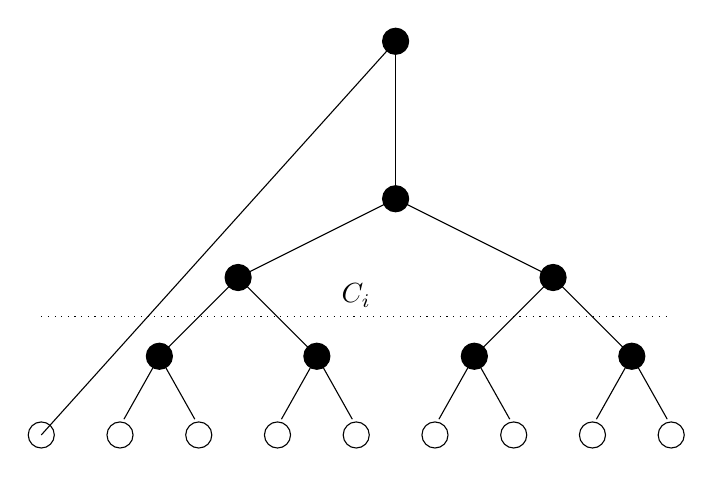
\begin{tikzpicture}
		\node[circle,draw] at (0,0) {};
		
		\node[circle,draw] at (1, 0){};
		\node[circle,draw,fill=black] at (1.5, 1){};
		\draw (1.5, 1) --(1.95, 0.2);
		\draw (1.5, 1) --(1.05, 0.2);
		\node[circle,draw] at (2,0) {};
		
		\node[circle,draw,fill=black] at (2.5, 2){};
		\draw (2.5, 2) --(1.5, 1);
		\draw (2.5, 2) --(3.5, 1);

		\node[circle,draw] at (3, 0){};
		\node[circle,draw,fill=black] at (3.5, 1){};
		\draw (3.5, 1) --(3.95, 0.2);
		\draw (3.5, 1) --(3.05, 0.2);
		\node[circle,draw] at (4,0) {};
		
		\node[circle,draw,fill=black] at (4.5, 3){};
		\draw (4.5, 3) --(2.5, 2);
		\draw (4.5, 3) --(6.5, 2);

		
		\node[circle,draw,fill=black] at (4.5, 5){};
		\draw (4.5, 5) --(4.5, 3);
		\draw (4.5, 5) --(0, 0);
		
		
		\node[circle,draw] at (5, 0){};
		\node[circle,draw,fill=black] at (5.5, 1){};
		\draw (5.5, 1) --(5.95, 0.2);
		\draw (5.5, 1) --(5.05, 0.2);
		\node[circle,draw] at (6,0) {};
		
		\node[circle,draw,fill=black] at (6.5, 2){};
		\draw (6.5, 2) --(5.5, 1);
		\draw (6.5, 2) --(7.5, 1);
		
		
		\node[circle,draw] at (7, 0){};
		\node[circle,draw,fill=black] at (7.5, 1){};
		\draw (7.5, 1) --(7.95, 0.2);
		\draw (7.5, 1) --(7.05, 0.2);
		\node[circle,draw] at (8, 0){};
		
		\draw[dotted] (0, 1.5) -- node[above] {$C_i$} (8, 1.5);
	\end{tikzpicture}
\caption{A hierarchical clustering tree of $n=9$ points. This tree contains the clustering $C_i$ described in the proof of Lemma \ref{lemma:treesOnX}.}
\label{fig:treeStructure}
\end{figure}
\end{proof}

\begin{restatable}{thrm}{VCDimT}
Given a finite set $\mc X$ and a finite class $\mc F = \{T_1, \ldots, T_s\}$ where each $T_i$ is a hierarchical clustering over $\mc X$. Then 
$$\vcdim({\mc F}) \le g(s)$$ where $g(s)$ is the smallest integer $n$ such that $\frac{\sqrt n!}{\lfloor \sqrt n/2 \rfloor! \enspace 2^{\lfloor \sqrt n/2 \rfloor}} \ge s $
\end{restatable}
\begin{proof}
Let $n$ be as defined in the statement of the theorem. Let $M^2 \subseteq \mc X^2$ be a set of size $> n^2$. Define $M := \{x: (x, y) \in M^2 \text{ or } (y, x) \in M^2\}$. We know that $|M| > n$. Using lemma \ref{lemma:treesOnX}, there exists a set of clusterings $\mc C = \{C_1, \ldots, C_{s'}\}$ of size $s' > \frac{n!}{\lfloor n/2 \rfloor! \enspace 2^{\lfloor n/2 \rfloor}} \ge s$ such that each $T_i \in \mc F$ contains atmost one $C_j \in \mc C$. Thus, there exists a clustering $C_j$ which is not captured by any $T_i \in \mc F$. Hence, $l_{\mc F}$ can't shatter any set of size $> n^2$.
\end{proof}


\section{Computation complexity of RCC for common clustering classes}
\label{section:efficientERM}

\RestyleAlgo{ruled}
\SetAlgoNoLine
\LinesNumbered
\SetNlSkip{-0.4em}
\begin{algorithm}[h]
\caption{ERM approach for a hierarchical clustering tree}
\label{alg:ERMTrees}
\Indp\KwIn{A set $X$, a set $ S \subseteq X^2$ labelled according to $C^*$. Given a clustering tree $T$ on $S_u = \{x: (x, y) \text{ or }  (y, x) \in S\}$.}
\KwOut{A clustering $\hat C \in T$ which implements ERM over $T$.}

\vspace{0.1in} Initialize $e(\nu) = a(\nu) = 0$ for all the leaf nodes $\nu$. \\
\For{all non-leaf nodes $\nu$ (in a bottom-up manner)}{\label{algLine:forNode}
Let $\nu_l$ be left sub-tree and $\nu_r$ the right sub-tree.\\
Initialize $s_a = d_a = 0$.\\
	\For{$(x, y) \in S$}{
	  \If {$x, y \in nl(\nu)$ and $C^*(x, y) = 0$}{
	      $d_a = d_a + 1$.
	  }
	  \If {$!(x \in nl(\nu_l)$ and $ y \in nl(\nu_r))$ and $!(y \in nl(\nu_l)$ and $ x \in nl(\nu_r))$}{\label{algLine:IfCondn}
		\textbf{continue}
	}
	\If {$C^*(x, y) = 1$}{
		$s_a = s_a + 1$.
	}
}
$a(\nu) = d_a$ \label{algLine:all}\\
$e(\nu) = \min \{e(\nu_l)+e(\nu_r)+s_a, a(\nu)\}$ \label{algLine:best}
}
\end{algorithm}

Alg. \ref{alg:ERM} described the general ERM approach to find the `best' clustering for any class $\mc F$ of clusterings. Consider the case when $\mc F = \{C_1, \ldots, C_s\}$ (a finite list of clusterings). Then to implement Alg. \ref{alg:ERM}, we first sample a set $S \subseteq X^2$ and then compute the error of each clustering on this set $S$. Computing the error of a clustering on $S$ takes $\Theta(|S|)$ time. Hence, for finite $\mc F$, the ERM approach can be implemented in time $\Theta(|\mc F| |S|)$. 

Now, let's focus on the case when $\mc F = \{T_1, \ldots, T_s\}$ (a finite set of clustering trees). Each tree $T_i$ can contain exponentially many clusterings. Hence, it is not clear if we can still implement the ERM approach in polynomial-time. Consider the problem of implementing the ERM approach when $\mc F = \{T\}$. The goal is to find the pruning in the tree which minimizes the loss $\hat L$. Given tree $T$, the clustering with the smallest loss is either the clustering which assigns all the points to a single cluster or the clustering with the best loss in $T_l$ (left subtree) concatenated with the clustering with the best loss in $T_r$ (right subtree). Before we describe our approach lets introduce a bit of notation.

For every node $\nu$ in the hierarchical clustering tree, let $nl(\nu)$ be the leaves which are descendants of $\nu$. For a leaf node $\nu$, $nl(\nu) = \{\nu\}$. Let $\mu_1 = \mu|S_-|$ and $\mu_2 = (1-\mu)|S_+|$. Let $$e(\nu) = \argmin_{C \in T_{\nu}} \mu_1|S_+|\hat P(C) + \mu_2|S_-|\hat N(C)$$ where $T_{\nu}$ is the tree $T$ restricted to the descendants of $\nu$. Let $a(\nu) = \mu_1|S_+|\hat P(C) + \mu_2|S_-|\hat N(C)$ where $C$ is the clustering which assigns all the descendants of $\nu$ to a single cluster. We are now ready tp describe our bottom-up approach in Alg. \ref{alg:ERMTrees}. Its easy to see that the running time of the approach is $\Theta(|S|^2)$. 

\section{Experimental evaluation}
\label{sec:evaluation}

\begin{table*}[t]
\centering
\resizebox{\textwidth}{!}{
\begin{tabular}{ |c || c|c||c|c|| c|c || c|c || c|c| } 
 \hline
  & \multicolumn{2}{c||}{\textbf{simulated}} & \multicolumn{2}{|c|}{\textbf{publications}} & \multicolumn{2}{c||}{\textbf{products I}} & \multicolumn{2}{c||}{\textbf{products II}} & \multicolumn{2}{c||}{\textbf{restaurants}}\\ \hline
Clustering & true loss & estimated loss & true loss & estimated loss & true loss & estimated loss & true loss & estimated loss & true loss & estimated loss \\ \hline
ArtPt           & 0.091         & 0.105         & 0.023         & 0.005         & 0.206         & 0.170         & 0.153         &   0.160           & 0.094	                        & 0.110 \\ \hline
Star            & 0.052         & 0.060         & 0.100         & 0.050         & 0.207	        & 0.190         & 0.231         &	0.170           & 0.041	                        & 0.045 \\ \hline
ApproxCorr      &  NA\footnote{ Algorithm did not finish within a reasonable time limit because of the high computational cost.}           & NA       & 0.180	        & 0.145         & 0.380	        & 0.310         & 0.373         &	0.340           & 0.094	                        & 0.065 \\ \hline
Markov          & 0.011         & \textbf{0.000}& 0.017	        & 0.010         & 0.159         & 0.130         & 0.125         &	0.085           & 0.045                         & 0.030 \\ \hline
Na\"iveDedup    & 0.397         & 0.365         & 0.497         & 0.495         & 0.413         & 0.405         & 0.394         &	0.380           & 0.094                         & 0.080 \\ \hline
C1 (single)     & 0.019         & 0.025	        & 0.016         & 0.018         & 0.150         & 0.110         & 0.131         &	0.120           & 0.022                         & \textbf{0.015} \\ \hline
C2 (complete)   & 0.005         & 0.005	        & 0.009	        & 0.009         & 0.150	        & 0.130	        & 0.135         &	0.065           & 0.034	                        & 0.040 \\ \hline
C3 (weighted)   & 0.002         & \textbf{0.000}& \textbf{0.005}& \textbf{0.006}& \textbf{0.110}& 0.110	        & 0.107         &	0.070           & \textbf{0.019}      & 0.020 \\ \hline
C4 (average)    & \textbf{0.001}& \textbf{0.000}& 0.007 	    & 0.017         & 0.120	        & \textbf{0.100}& \textbf{0.099}&	\textbf{0.060}  & \textbf{0.019}      & 0.020 \\ \hline \hline
Mean loss difference   &               & 0.016         &               & 0.014         &               & 0.027         &               &   0.035           &                        & 0.010 \\ \hline
\end{tabular}
}
\caption{True loss and the loss estimated by our framework.}
\label{tab:exp3}
\end{table*}

\begin{table}[t]
\centering
\resizebox{\textwidth}{!}{

\begin{tabular}{ |c|c|c|c|c|c|c|c|c| } 
\hline
  &  & \multicolumn{2}{|c|}{\textbf{25, 25 samples}} & \multicolumn{2}{|c|}{\textbf{100, 100 samples}} & \multicolumn{2}{|c|}{\textbf{500, 500 samples}} \\ \hline
Clustering & true loss & \# queries & estimated loss & \# queries & estimated loss & \# queries & estimated loss \\ \hline
C1 (single) & \textbf{0.06107}   &  51 & 0.06 & 204	&   0.025 & 1023 &	0.024   \\ \hline
C2 (complete) &	\textbf{0.04177} &	50 & 0.02 &	210 &	0.005 & 1024 &	0.016 \\ \hline
C3 (weighted) & \textbf{0.03831} &	50 & 0.02 &	203 &	0.015 &	1027 &	0.016 \\ \hline
C4 (average) &	\textbf{0.03489} &	52 & 0.02 &	207 &	0.020 &	1043 &	0.013 \\ \hline
\end{tabular}

}
\caption{Simulated dataset: Impact of number of samples on the loss of the clustering}
\label{tab:exp1}
\end{table}




\begin{table}[t]
\centering
\resizebox{\textwidth}{!}{

\begin{tabular}{ |c|c|c|c|c|c|c|c|c| } 
 \hline
  &  & \multicolumn{2}{|c|}{\textbf{25, 25 samples}} & \multicolumn{2}{|c|}{\textbf{100, 100 samples}} &  \multicolumn{2}{|c|}{\textbf{500, 500 samples}} \\ \hline
Clustering & true loss & \# queries & estimated loss & \# queries & estimated loss & \# queries & estimated loss \\ \hline
C1 (single) & \textbf{0.11075}   &  51 & 0.08 & 208 &	0.055 &	1031 &	0.041 \\ \hline
C2 (complete) &	\textbf{0.37172} &	50 & 0.34 &	204 &	0.315 &	1035 &	0.334 \\ \hline
C3 (weighted) & \textbf{0.29622} &	51 & 0.14 &	203 &	0.260 &	1037 &	0.239 \\ \hline
C4 (average) &	\textbf{0.26877} &	50 & 0.20 &	204 &	0.195 &	1027 &	0.202 \\ \hline
\end{tabular}

}

\caption{Publications dataset: Impact of number of samples on the loss of the clustering}
\label{tab:exp2}
\end{table}

\begin{figure}[t]
    \centering
    \begin{subfigure}[t]{0.5\textwidth}
        \centering
        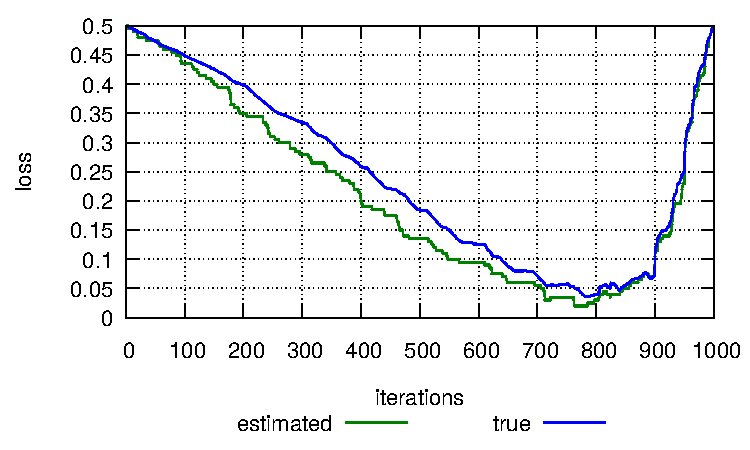
\includegraphics[trim=100 0 100 0, width=0.5\linewidth,valign=t]{figures/deDuplication/plot_simulated_s.pdf}
        \caption{Single linkage}
    \end{subfigure}%
    ~ 
    \begin{subfigure}[t]{0.5\textwidth}
        \centering
        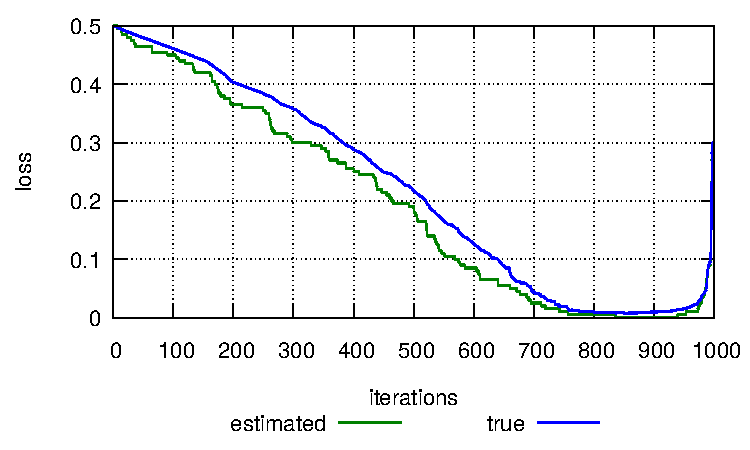
\includegraphics[trim=100 0 100 0, width=0.5\linewidth,valign=t]{figures/deDuplication/plot_simulated_c.pdf}
        \caption{Complete linkage}
    \end{subfigure}
	\caption{Simulated dataset: Loss reported for every iteration of hierarchical clustering}
    \label{fig:simulated}
\end{figure}

\begin{figure}[t]
    \centering
    \begin{subfigure}[t]{0.5\textwidth}
        \centering
        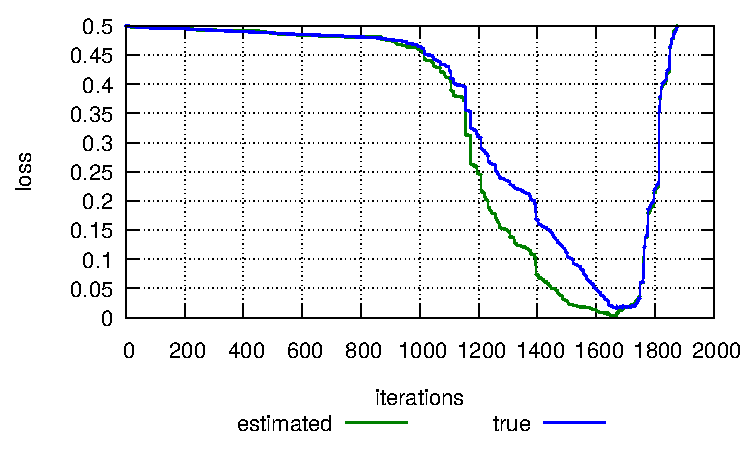
\includegraphics[trim=100 0 100 0, width=0.5\linewidth,valign=t]{figures/deDuplication/plot_real_s.pdf}
        \caption{Single linkage}
    \end{subfigure}%
    ~ 
    \begin{subfigure}[t]{0.5\textwidth}
        \centering
        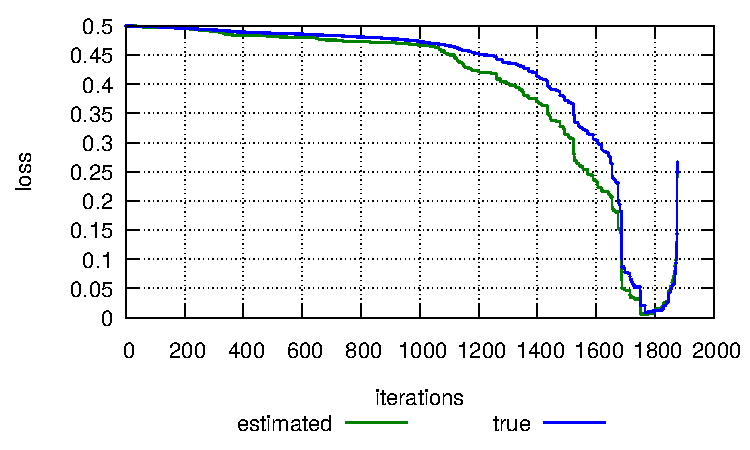
\includegraphics[trim=100 0 100 0, width=0.5\linewidth,valign=t]{figures/deDuplication/plot_real_c.pdf}
        \caption{Complete linkage}
    \end{subfigure}
	\caption{Publications dataset: Loss reported for every iteration of hierarchical clustering}
    \label{fig:publications}
\end{figure}

\begin{figure}[t]
    \centering
    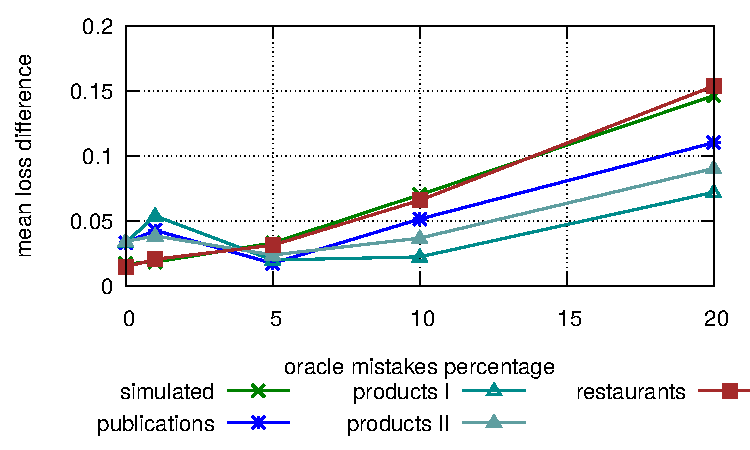
\includegraphics[trim=0 0 0 0, width=\linewidth,valign=t]{figures/deDuplication/plot_oracle_error.pdf}
    \caption{Impact of oracle mistakes}
    \label{fig:oracle-error}
\end{figure}
    



We now present the evaluation of our framework on a simulated and four real world datasets.
In Section \ref{sec:exp1} we show that our framework is generic and can be used to choose amongst many of the classes of algorithms for de-duplication. We also show that our framework can always choose a clustering which is close to the best clustering (algorithm) from a given class of clustering (algorithms) and our estimated loss for each of the clustering is very close to the true loss of these clustering algorithms.
In Section \ref{sec:exp2} we show that our framework is robust to upto 10\% of oracle mistakes, which far exceeds the intended settings dealing with human experts.
Finally, in Section \ref{sec:exp3} we show that in our framework a relatively small number of samples are enough to accurately estimate the loss of a clustering.

\subsection{Evaluation setup}
\label{sec:setup}
\textbf{Algorithms} In our evaluation we use four graph based clustering algorithms: (1) Articulation point clustering (\textit{ArtPt}) \cite{cormen2009introduction}, (2) Star clustering (\textit{Star}) \cite{aslam2006star}, (3) Approximate correlation clustering (\textit{ApproxCorr}) \cite{bansal2004correlation}, (4) Markov clustering (\textit{Markov}) \cite{van2000graph}. These graph based algorithms have been used for de-duplication problems as shown in previous work \cite{hassanzadeh2009framework}.
Hierarchical clustering algorithms are very effective and have been widely used to perform de-duplication. We consider 4 different linkage methods for hierarchical clustering: single linkage (C1), complete linkage (C2), weighted linkage (C3), and average linkage (C4). 
In addition to this we also implemented a heuristic based de-duplication algorithm (\textit{Na\"iveDedup}) where any two data points are considered similar if their distance is below a certain threshold. The output of this algorithm is pairs of data points which are marked similar.

\textbf{Datasets} For our evaluation we use five datasets.
First dataset is a simulated dataset of ten thousand strings of length 20 where we simulate a clustering over the set of strings and use it as our ground truth.
We use Jaro distance \cite{jaro1980unimatch} as the distance metric for strings.
To simulate a clustering we generate some seed strings and then for each seed string we generate multiple secondary strings by slightly editing the seed string.
Each cluster of strings resembles a single entity.
Second dataset is a real-world bibliographical information of scientific publications \cite{pubdata}.
The dataset has 1879 publication records with duplicates.
The ground truth of duplicates is available.
To perform clustering on this dataset we first tokenized each publication record and extracted 3-grams from them.
Then, on 3-grams we used Jaccard distance to define distance between two records.
Next two datasets are lists of E-commerce products: First dataset contains 1,363 products from Amazon, and 3,226 products from Google, and the ground truth has 1,300 matching products.
Second dataset contains 1,082 products from Abt, and 1,093 products from Buy, and the ground truth has 1,098 matching products. Both these products datasets are publicly available at \cite{products}. 
The fifth dataset is a list of 864 restaurants from the Fodor's and Zagat's restaurant guides that contains 112 duplicates. This dataset is also publicly available at \cite{restaurant}.
To perform clustering on the products and restaurants datasets we normalized the records (product or restaurant description) using standard techniques from natural language processing, namely; denoising text, word tokenization, normalization, and stemming and lemmatization. Given a record, this process gives us a list of word tokens. For each token, we first obtained a vector representation of the word using  \textit{Global Vectors} for word representations (GloVe \cite{jeffrey2014glove}). We averaged this representation across word tokens to obtain the representation of a single record. We use cosine similarity to define the distance between two records.
For the simulated and publications datasets, our distance metric was Jaccard and hence we use the MinHash \cite{broder2000min} as the hashing scheme. For the rest of the datasets, we used SimHash \cite{charikar2002similarity} as the hashing scheme. 
For all the datasets we use ground truth as the oracle that can answer \textit{same-cluster queries}. 
To calculate the true loss of a clustering (i.e. $L_{C^*}(C)$) we access all of the ground truth. Our framework uses only a sample of the ground truth to estimate the loss of a clustering.
To judge the performance of our framework we compare the estimated loss $\hat L_{C^*}(C)$ against the true loss.

\subsection{Clustering selection}
\label{sec:exp1}
In this experiment we demonstrate that our framework is generic and can be used to choose the best clustering algorithm amongst any of the classes of algorithms for de-duplication.
We used our framework on all the algorithms mentioned in Section \ref{sec:setup}. The results on five datasets are summarized in Table \ref{tab:exp3}. For each dataset we report the loss of the true-best clustering ($L_{C^*}(C)$) and the estimated loss of the best clustering selected by our framework $\hat L_{C^*}(C)$.
This experiment highlights two main features of our framework: (i) our framework can always choose a clustering close to the best clustering  algorithm from a given class of clustering algorithms using only a small number of samples, which is 200 (100 positive samples, and 100 negative samples) for all datasets and all the algorithms in Table \ref{tab:exp3}. (ii) Our estimated loss for each clustering is very close to the true loss of these clustering algorithms. At the bottom of the table we report the mean loss difference between estimated loss and true loss computed over all the algorithms. 

We would also like to emphasize that in our framework we sample only once for each dataset and use that  sample to estimate the loss of all the clusterings. In Figure \ref{fig:simulated} and \ref{fig:publications} we show that our sample can very closely estimate the loss of every clustering generated at each iteration of the hierarchical clustering. Similarly, for Table \ref{tab:exp3} we sampled only once for each dataset and evaluated all the clusterings generated by each algorithm.
Note that, each of the graph based algorithms have a hyper-parameter, i.e. the threshold on the edge weights. Edges with weights above this threshold represent dissimilar items and are pruned from the graph. For each of the graph based clustering algorithm we applied our framework on multiple values of the hyper-parameter and report only the ones with least true loss. However, for every choice of the hyper-parameter we observed that the estimated loss was very close to the true loss.

\subsection{Effect of oracle mistakes}
\label{sec:exp2}
In this experiment we show that our framework is effective in real-world scenarios where the oracle may not be perfect and can make mistakes. Whenever the oracle classifies a similar pair as dissimilar or a dissimilar pair as similar we count it as a mistake. In our datasets we artificially introduce such mistakes and vary their ratio from from 0\%, to 20\%. In Figure \ref{fig:oracle-error} we show that our framework can closely estimate the clustering loss up to 10\% of oracle mistakes, which, in real-world far exceeds the intended settings dealing with human experts. The Y-axis in Figure \ref{fig:oracle-error} reports the mean difference between true loss and estimated loss over all the clusterings selected in Table \ref{tab:exp3}.

%on four different methods of hierarchical clustering (C1 - C4). For each clustering, the goal is to find the pruning from the clustering tree that has minimum loss. We compare the loss of the best clustering found by our framework against the loss of the true-best clustering. We find the loss of the true-best clustering by performing all $|X|^2$ queries against the ground truth. In Table \ref{tab:exp3} we report the loss of the best clustering for all four clustering methods and both the datasets. In all the scenarios the best clustering picked by our framework is very close to the true-best clustering. The framework used 100 positive and 100 negative samples for this experiment for both the datasets. In Figures \ref{fig:simulated} and \ref{fig:publications}, we report the loss at every iteration of the hierarchical clustering. The loss reported by our framework is always close to the true loss of the clustering at every iteration. Another important point to note is that by only sampling 200 points, we are able to estimate the loss of all the clusterings (or prunings) of the hierarchical clustering tree.

\subsection{Impact of sample size}
\label{sec:exp3}

In this experiment we show that even a small number of samples are enough to estimate the true loss ($L_{C^*}(C)$).
%The true loss is computed by querying every pair $(x_1, x_2) \in X^{[2]}$ against the oracle (ground truth in our case).
We consider four different clusterings, each one picked at random from the four hierarchical clustering methods (C1 - C4).
Table \ref{tab:exp1} and \ref{tab:exp2} reports the loss for simulated and publications dataset, respectively.
For each dataset we increased the number of positive and negative samples and measured the loss.
The table also shows the true loss of the clustering.
It can be seen that the estimated loss calculated by our framework is close to the true loss even with 25 positive samples and 25 negative samples.
In addition to this, the loss does not change much by increasing the number of samples.
Which means that there is no incentive to sample more.
We also show that the number of queries performed by our framework are close to the sample size (as claimed in Thm. \ref{thm:queryComplexity}), which are orders of magnitude less than $O(|X|^2)$.
For example, in the simulated dataset and single linkage clustering (C1) with 25 positive and 25 negative samples our framework performed 51 queries, that means only one query was wasted. Similarly, 4 queries were wasted for 100 positive and 100 negative samples, and so on.

 
\ifdefined\COMPLETE
\else
\end{document}
\fi

